\documentclass[conference]{IEEEtran}
\IEEEoverridecommandlockouts

\usepackage[T1]{fontenc}
\usepackage{cite}
\usepackage{amsmath,amssymb}
\usepackage{graphicx}
\usepackage{booktabs}
\usepackage{xcolor}
\usepackage{url}
\usepackage{tikz}
\usetikzlibrary{positioning,arrows.meta}

% Grey TODO notes. To hide them all for the final version, change the line below to
% \newcommand{\todo}[1]{}
\newcommand{\todo}[1]{}

\graphicspath{{figures/}}

\begin{document}

\title{ICARUS: Solar Storms and Satellite Decay\\
\large A Causal Analysis of Geomagnetic Storm Effects on Low-Earth-Orbit Objects}

\author{
\IEEEauthorblockN{Sonu Akash}
\IEEEauthorblockA{PES1UG24AM908\\PES University}
\and
\IEEEauthorblockN{Siddanth Anil}
\IEEEauthorblockA{PES1UG24AM274\\PES University}
\and
\IEEEauthorblockN{Sidhant Holla}
\IEEEauthorblockA{PES1UG24AM466\\PES University}
\and
\IEEEauthorblockN{Piyush Shiv}
\IEEEauthorblockA{PES1UG24AM191\\PES University}
}

\maketitle

\begin{abstract}
Geomagnetic storms heat and swell the upper atmosphere, so satellites in low Earth orbit (LEO)
fall faster. We measure how much faster, how well NRLMSIS~2.1 predicts it, and how much of the
loss operators win back. We used
one year of public two-line element sets (April 2024 to April 2025), which covers 20 storms with
Dst below $-50$~nT including the May 2024 superstorm, for 250 passive objects (debris and rocket
bodies) between 400 and 800~km. We compare each object's decay with a physics baseline that
already uses the measured solar flux (F10.7) and treat each storm as a natural experiment. A
stacked event study finds that storms speed up decay by 14.1~m/day over days 0--2 after onset
(95\% CI 8.4--19.8), and double machine learning gives 0.39~m/day for every nT of ap. Reading
these as causal effects assumes no time-varying confounding is left after our adjustment. Pooled
over days 0--2, NRLMSIS~2.1 shows little error but under-predicts decay at peak activity, and in
the three largest storms its errors go in different directions. A causal forest shows that the damage
scales with drag sensitivity times an altitude factor that falls about threefold from 620 to
750~km. In an exploratory look at 21 Starlink satellites, the observed orbits are consistent
with an almost complete offset of the predicted storm loss (offset ratio 1.17, 95\% CI
0.97--1.36), almost all during the storm. Placebo dates, a pre-trend test, a high-altitude control and
a simulator with a planted effect back the storm-effect estimate.
\end{abstract}

\begin{IEEEkeywords}
geomagnetic storms, orbital decay, thermospheric density, NRLMSIS, causal inference,
double machine learning, event study, causal forest, space situational awareness
\end{IEEEkeywords}


% Section order and owners (see README.txt):
\section{Introduction}
\label{sec:intro}

In February 2022 SpaceX launched 49 Starlink satellites into a low parking orbit. Right after launch a
minor geomagnetic storm arrived, the air at that altitude became denser, and 38 of the
satellites were dragged back into the atmosphere before they could climb
away~\cite{fang2022starlink}. Two years later, the May 2024 ``Gannon'' storm, the strongest in
about twenty years, sped up the decay of almost every tracked object in low Earth orbit and set
off a wave of manoeuvres by operators~\cite{parker2024gannon}. Drag decides how long each of
the tens of thousands of objects in LEO stays up, storms can change it within hours, and
collision screening and re-entry forecasts depend on getting it right.

The physics is well known. During a storm, energy from the solar wind is dumped into the upper
atmosphere at high latitudes. The thermosphere heats and expands, the density at a given height
goes up, and so does drag. Putting a number on the storm's effect is harder than it sounds,
though, because the Sun also changes the atmosphere in a slower way. Its ultraviolet (UV)
output, tracked by the F10.7 radio flux, heats the thermosphere too, and periods with high UV
also tend to have more storms. If we simply correlate storm strength with decay, part of the UV
effect gets credited to the storms. On top of that, operators predict density with empirical
models such as NRLMSIS~\cite{picone2002nrlmsise,emmert2021nrlmsis,emmert2022msis21}, so it
matters just as much whether these models are wrong during storms.

Our approach is to treat each storm as a natural experiment. Nobody can schedule when a storm
arrives, so if we adjust for the measured F10.7 and the season, the decay just before a storm
and the decay just after it should differ only because of the storm. This is a causal reading,
and it rests on one assumption: that no time-varying confounder is left after the adjustment.
Our placebo and control checks support that assumption but cannot prove it. We use only passive
objects (debris and rocket bodies) in the main analysis, because they cannot fire thrusters and
their orbits change only through natural forces. We also measure their decay against a physics
baseline that already includes the real F10.7, so much of the UV effect is removed before any
statistics are run.

We ask three questions.
\textbf{Q1:} How much extra decay do storms cause, and how wrong is NRLMSIS~2.1 during them?
\textbf{Q2:} Which objects are hit hardest, by altitude, inclination and drag sensitivity?
\textbf{Q3:} How much of the storm's altitude loss do operators undo, during the storm and
after it?

To answer them we built a 250-object passive cohort covering 20 storms and estimated the storm
effect two ways, with a stacked event study and with double machine learning, which agree. We
estimated the NRLMSIS~2.1 storm-time error separately and checked the three largest storms
with a calm-to-calm comparison that does not depend on how TLE fits spread a loss across days.
A causal forest turned the per-object effects into a vulnerability map, and for Starlink we
built an exploratory offset ratio that splits the operator response into a part during the
storm and a part afterwards. Every estimator was tested on a simulator with a planted effect.

Sections~\ref{sec:related} to~\ref{sec:design} cover related work, data, the physics baseline
and the causal design, Sections~\ref{sec:q1} to~\ref{sec:q3} answer the three questions,
Section~\ref{sec:robust} tries to break the results and Section~\ref{sec:discussion} discusses
their limits.
   % Anil
\section{Related Work}
\label{sec:related}

\textit{Storm-time drag.} Oliveira and Zesta~\cite{oliveira2019drag} used accelerometer-derived
densities to measure satellite drag during magnetic storms and showed that decay grows with
storm intensity and duration. Fang et al.~\cite{fang2022starlink} reconstructed the February
2022 Starlink loss and found that pre-launch estimates based on NRLMSISE-00 underestimated the
drag compared with a coupled whole-atmosphere model. Parker and Linares~\cite{parker2024gannon}
looked at TLEs of the whole LEO catalogue during the May 2024 storm and documented both the
density increase and the large manoeuvre response. Basak et al.~\cite{basak2024cosmicdance}
lined up hourly Dst with Starlink TLEs and showed that even moderate storms can shift satellite
altitudes, and their follow-up, CosmicDancePro~\cite{basak2026cosmicdancepro}, studies how the
fleet was managed during the May 2024 superstorm. Wu et al.~\cite{wu2025decay} calibrate an
orbital decay factor on quiet periods and combine it with a density proxy to track storm-time
decay in near real time. Bruinsma and Laurens~\cite{bruinsma2024storms} test thermosphere models
over 152 storms, but against the accelerometer densities of a few science satellites, not the
decay of a tracked cohort. Most of these decay studies look at one storm, one satellite or one
constellation.

\textit{Density models.} NRLMSISE-00~\cite{picone2002nrlmsise} and its successors NRLMSIS
2.0~\cite{emmert2021nrlmsis} and 2.1~\cite{emmert2022msis21} compute density from F10.7, its
81-day mean and the ap index. Their storm-time accuracy is usually judged against a few
accelerometer-carrying satellites. We judge NRLMSIS~2.1 by the decay it predicts for 250
objects, which is the number operators actually use.

\textit{Causal machine learning.} Double machine learning~\cite{chernozhukov2018dml} estimates a
treatment effect after flexible models have removed the confounders, using cross-fitting to
avoid overfitting bias. Causal forests~\cite{wager2018forest,athey2019grf} extend this to
effects that vary with covariates. Event studies with staggered events and clean
controls~\cite{cengiz2019stacked,sun2021eventstudy,callaway2021did} avoid comparing against
units that are already treated. With only a few independent events, cluster-robust inference
needs small-sample fixes such as the wild cluster
bootstrap~\cite{cameron2008bootstrap,webb2023wild}.

\textit{Where this paper fits.} What we add is the combination. We look at many storms through
the decay of a whole tracked cohort, we restrict the main analysis to objects that cannot
manoeuvre, we estimate the total storm effect and the density-model error separately, and we
use calm-to-calm totals to tell a timing error apart from an error in the accumulated loss.
Every estimator is also tested on synthetic data with a known answer. The Starlink offset ratio
is an exploratory extra.
   % Holla
\section{Data}
\label{sec:data}

\subsection{Choosing the objects}
\label{sec:cohort}

The main sample is 250 passive objects between 400 and 800~km. We kept objects that appear on at
least eight of nine Space-Track snapshot dates and spread the sample across 100-km altitude bands
instead of picking by NORAD number, which gives 39, 63, 82 and 66 objects in the four bands. We
use debris and rocket bodies because they cannot correct their orbits. We also kept 15 objects
between 1,040 and 1,211~km as a high-altitude control group, since storms should barely touch
them. The first full download gave 205,145 deduplicated TLE states and 199,580 intervals between
neighbouring states: 188,560 in the main sample and 11,020 in the control group.

For the operator question we built a separate active cohort of 25 Starlink satellites and 25
other payloads, chosen with the same coverage rule. Their pipeline keeps station-keeping
intervals and does not remove climbs. The joined object catalogue has 291 objects.

\subsection{Cleaning the TLEs}
\label{sec:cleaning}

We parse each TLE with SGP4~\cite{vallado2006sgp4} and convert its (Kozai) mean motion to a mean
semi-major axis using the WGS-72 constants. Using SGP4's recovered (Brouwer) mean motion instead
shifts the semi-major axis by a nearly constant amount of up to about 3~km and changes decay
rates by 0.03\% over the cohort (at most 0.2\% for any object), so nothing depends on this choice. When the same epoch was published
more than once we keep only the latest record, so that re-issues do not create fake intervals of
zero or near-zero length.

One point needs care, and a reviewer of our project proposal raised it directly. TLEs are mean
elements fitted to a day or more of tracking. They are not measured positions, so when we say
``altitude'' we mean the mean semi-major axis minus Earth's equatorial radius, not a true
geometric height. SGP4 fitting artifacts and changes in eccentricity can both create altitude
drops that never happened, and a storm study is exactly where such fake drops would do the most
harm. We defend against them in three ways. First, we track the mean semi-major axis rather than
perigee height, which swings with eccentricity, and we keep only near-circular orbits
(eccentricity below 0.01). Second, we reject states outside the altitude bounds, cross-tag
jumps, pairs that fail the TLE consistency checks at either end, and isolated jumps caught by a
Hampel filter. Third, for the largest storms we also compare calm-to-calm totals
(Section~\ref{sec:extreme}), which do not depend on how a fit spreads a loss across days.

Neighbouring clean states form an interval. We drop intervals that straddle a storm onset,
because they cannot be called either before or after the storm; 5,300 were dropped this way.
Four intervals were longer than five days (the longest 7.1 days), and we kept and reported them
rather than quietly removing them. The cross-tag and rolling-median checks flagged no objects.

TLE noise can make an object appear to climb a little. We estimate each object's noise level
from local median absolute deviations and flag such climbs, but keep them in the table, because
deleting only the upward steps would bias decay downwards. Dropping them anyway moves the
short-run storm effect only from $-14.1$ to $-14.6$~m/day. The outlier step is a Hampel filter
on the NRLMSIS~2.1 residual, with a five-day window and $k = 3.5$. It flags 11,005 passive
intervals in all (5.5\%), and these are left out of every analysis. In the main sample, 178,107
of the 188,560 intervals pass and form the analysis sample. Table~\ref{tab:cleaning} lists the steps.

\begin{table}[t]
\caption{TLE cleaning steps (passive cohort, first download)}
\label{tab:cleaning}
\centering
\small
\begin{tabular}{@{}p{2.55cm}p{2.45cm}p{2.5cm}@{}}
\toprule
Step & Affected & Treatment \\
\midrule
Deduplication & 205,145 states kept & Keep latest re-issue \\
Storm-onset bridge & 5,300 intervals & Dropped \\
Gap $>$5 days & 4 (max 7.1 d) & Reported, kept \\
Cross-tag check & 0 objects & None removed \\
Rolling median & 0 objects & None removed \\
Climb diagnostic & 4,705 intervals & Kept, flagged \\
Hampel filter & 11,005 (5.5\%) & Excluded \\
\bottomrule
\end{tabular}
\end{table}

The outcome for each interval is the change in semi-major axis divided by the elapsed time, in
metres per day, so a negative number means the object is coming down. Each row also carries the
storm it belongs to, its day relative to that storm's onset, its cleaning flags, altitude band
and object role, so every analysis applies the same exclusions without going back to the raw
TLEs.

\subsection{Do TLEs see storm decay?}
\label{sec:precise}

Before trusting TLEs, we compared them with precise orbits from GRACE-FO-1~\cite{landerer2020gracefo}
and Swarm-A~\cite{friis2006swarm}. These products give position and velocity directly. We turn
them into an osculating semi-major axis with the vis-viva equation, average over whole orbits and
then compute daily decay rates. For Swarm-A we measure the orbital period from successive radius
minima (93.83~min) instead of assuming it, and we remove duplicate timestamps at file boundaries.

The October 2024 GRACE-FO comparison is the clearest test. The TLE and precise decay rates peak
on the same day, correlate at about 0.70 with no lag, and have a similar storm-day size (about
$-0.10$ against $-0.12$~km/day). So TLEs catch the timing and most of the size of storm decay,
while slightly underestimating the peak. Over 19 days in May 2024, the semi-major-axis levels
agree with a centred correlation of 0.907, a centred RMSE of 0.097~km and a slope difference of
0.0025~km/day once the mean-versus-osculating offset is removed. Swarm-A gives a weaker
zero-lag correlation of 0.457. Its product and sampling are different, so we treat it as a
supporting check rather than pooling it with GRACE-FO. Together they show the cleaned TLE intervals are good enough for a cohort
study.

\subsection{Space weather and the storm list}
\label{sec:sw}

Space-weather data come from NASA OMNIWeb: the planetary index ap (3-hourly and linear in
disturbance, so it can be averaged), the Dst index, Kp, and the daily F10.7 flux with its 81-day
centred mean. We measure storm strength with ap or Dst and never average Kp, which is
quasi-logarithmic.

We call any period with Dst below $-50$~nT a storm and merge dips less than three days apart.
For each storm we record the main-phase onset (the hour of highest Dst in the 24~h before the
minimum), the minimum Dst, and the recovery end (the first hour after the last sub-$-50$~nT hour
at which Dst climbs back above $-30$~nT). By minimum Dst, storms are moderate ($-50$ to
$-100$~nT), strong ($-100$ to $-200$), severe ($-200$ to $-350$) or extreme (below $-350$). Our
window has 20 storms: 11 moderate, 6 strong, 2 severe (October 2024 and 31 December 2024) and 1
extreme (May 2024, Dst $-406$~nT). Day~0 is always the main-phase onset, and the event window
runs from day $-10$ to day $+20$.

Fig.~\ref{fig:may} shows the raw signal: around the May 2024 storm, the median
decay rate of the 250 passive objects goes from $-18$~m/day three days before onset to
$-60$~m/day on the first day after it.

\begin{figure}[t]
\centering
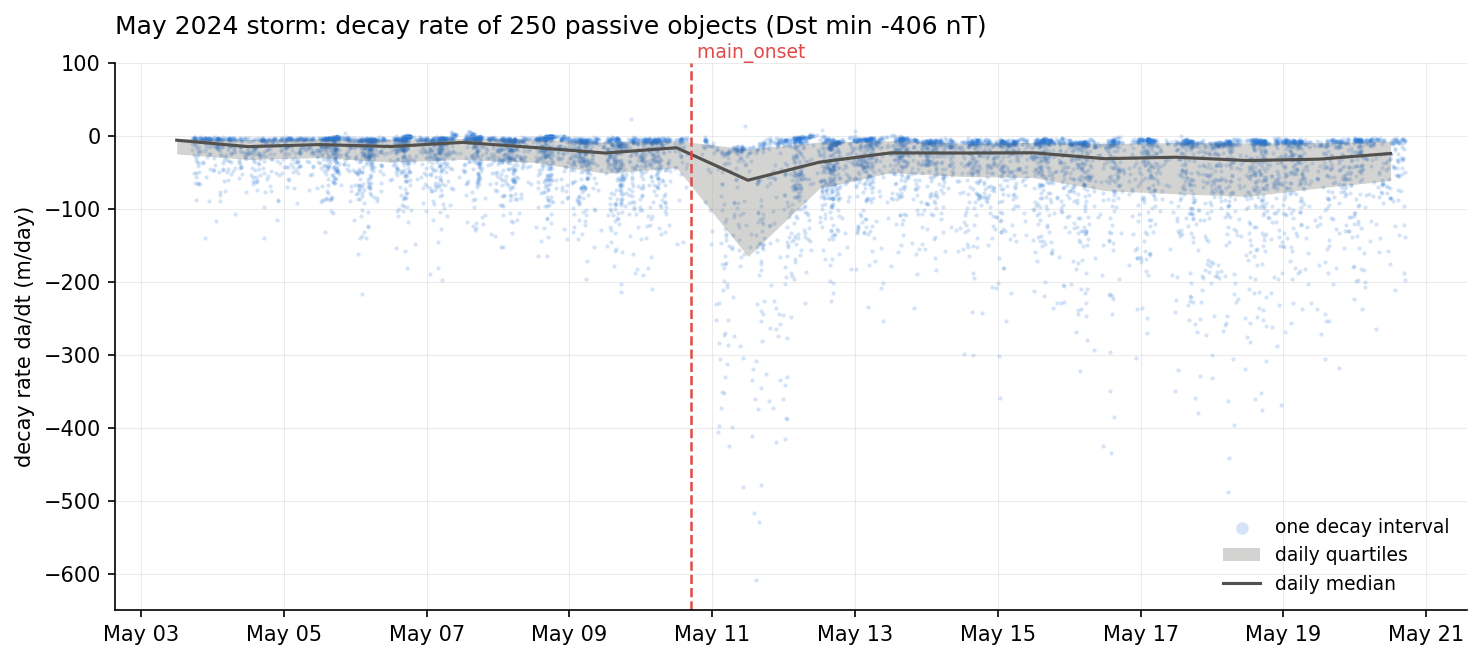
\includegraphics[width=\columnwidth]{fig1_may2024_cohort.png}
\caption{Median decay rate of the 250 passive objects around the May 2024 storm. Decay
increases about 3.4-fold on the first day after main-phase onset.}
\label{fig:may}
\end{figure}
           % Piyush (done) + Sonu (space weather)
\section{Physics Baseline and Outcomes}
\label{sec:physics}

\subsection{What physics predicts}
For a
near-circular orbit, drag shrinks the semi-major axis $a$ at the rate
\begin{equation}
\frac{da}{dt} = -B\,\rho\,\sqrt{\mu a}, \qquad B = \frac{C_D A}{m},
\label{eq:drag}
\end{equation}
where $\rho$ is the neutral mass density, $\mu$ is Earth's gravitational parameter and $B$ is
the object's drag sensitivity (m$^2$/kg). For every interval we propagate the orbit with SGP4 at
evenly spaced times, half from each end's TLE, and look up $\rho$ along the track with
NRLMSIS~2.1~\cite{emmert2022msis21}, using NRLMSISE-00~\cite{picone2002nrlmsise} as a robustness
check. The model is driven by the observed F10.7, its 81-day mean and the 3-hourly ap history.
The interval's density driver is $D = -\overline{\rho\sqrt{\mu a}}$, and the predicted decay is
$B\,D$.

We do not take $B$ from a catalogue. Instead we fit it for each object on quiet intervals away
from any storm, as a $\Delta t$-weighted ratio of sums,
$\hat B = \sum_i \dot a_i \Delta t_i / \sum_i D_i \Delta t_i$, using every other quiet interval
and holding the rest back for validation. Before the fit, a Hampel filter on the residual
(five-day window, $k=3.5$) removes bad TLE pairs. A weekly block bootstrap puts the median
standard error of $\hat B$ at 3\% (maximum 8\%), and no object breaks the instability rule we
set in advance (fewer than 30 fit intervals, a standard error above 25\% of $\hat B$, or an
interval reaching zero).

\subsection{Two outcomes}
From the same observed decay $\dot a^{\text{obs}}$ we build two outcomes, both in m/day:
\begin{align}
Y_{\text{total}} &= \dot a^{\text{obs}} - \hat B\,D(\text{F10.7},\,ap_{\text{quiet}}),\\
Y_{\text{residual}} &= \dot a^{\text{obs}} - \hat B\,D(\text{F10.7},\,ap).
\end{align}
$Y_{\text{total}}$ runs the model with ap held at the storm's pre-storm quiet value (the median
ap over days $-10$ to $-3$). It asks what the storm did beyond a calm atmosphere, so it measures
the \emph{total storm effect}, and it is the outcome we read causally. $Y_{\text{residual}}$ uses
the real ap, so it asks what NRLMSIS~2.1 missed and measures the \emph{model error}. Strictly,
it also soaks up any storm-time change in the drag coefficient and any leftover TLE artifacts,
so it is model error in that broad sense. In both outcomes F10.7 stays at its real value, so the
baseline already accounts for UV before any statistics, and negative values mean more decay
than the baseline. Air density sits on the path from storm to decay
(storm $\rightarrow$ density $\rightarrow$ drag), so it enters only through this baseline and is
never used as a control.

\subsection{Does the baseline work?}
On the 50,674 held-out quiet intervals the mean NRLMSIS~2.1 residual is $-0.13$~m/day, with a
weekly-block standard error of 1.07~m/day, against a mean decay of $-50.6$~m/day. The per-object $t$-statistics have a
standard deviation of 0.82, and 6 of 250 objects have $|t|>2$, about what chance alone would
give. For the 116 rocket bodies with a DISCOSweb mass and cross-section, our fitted $\hat B$
ranks the objects the same way as the catalogue value $2.2\,A/m$ (Spearman $\rho = 0.81$,
Fig.~\ref{fig:valid}). These bodies come from about 15 stage types, so this is really a check
on stage types, not on 116 independent points. Fitted $\hat B$ is about 0.8 times the catalogue
value, which fits an orientation-averaged cross-section, so we only use the ranking as
validation.

\begin{figure}[t]
\centering
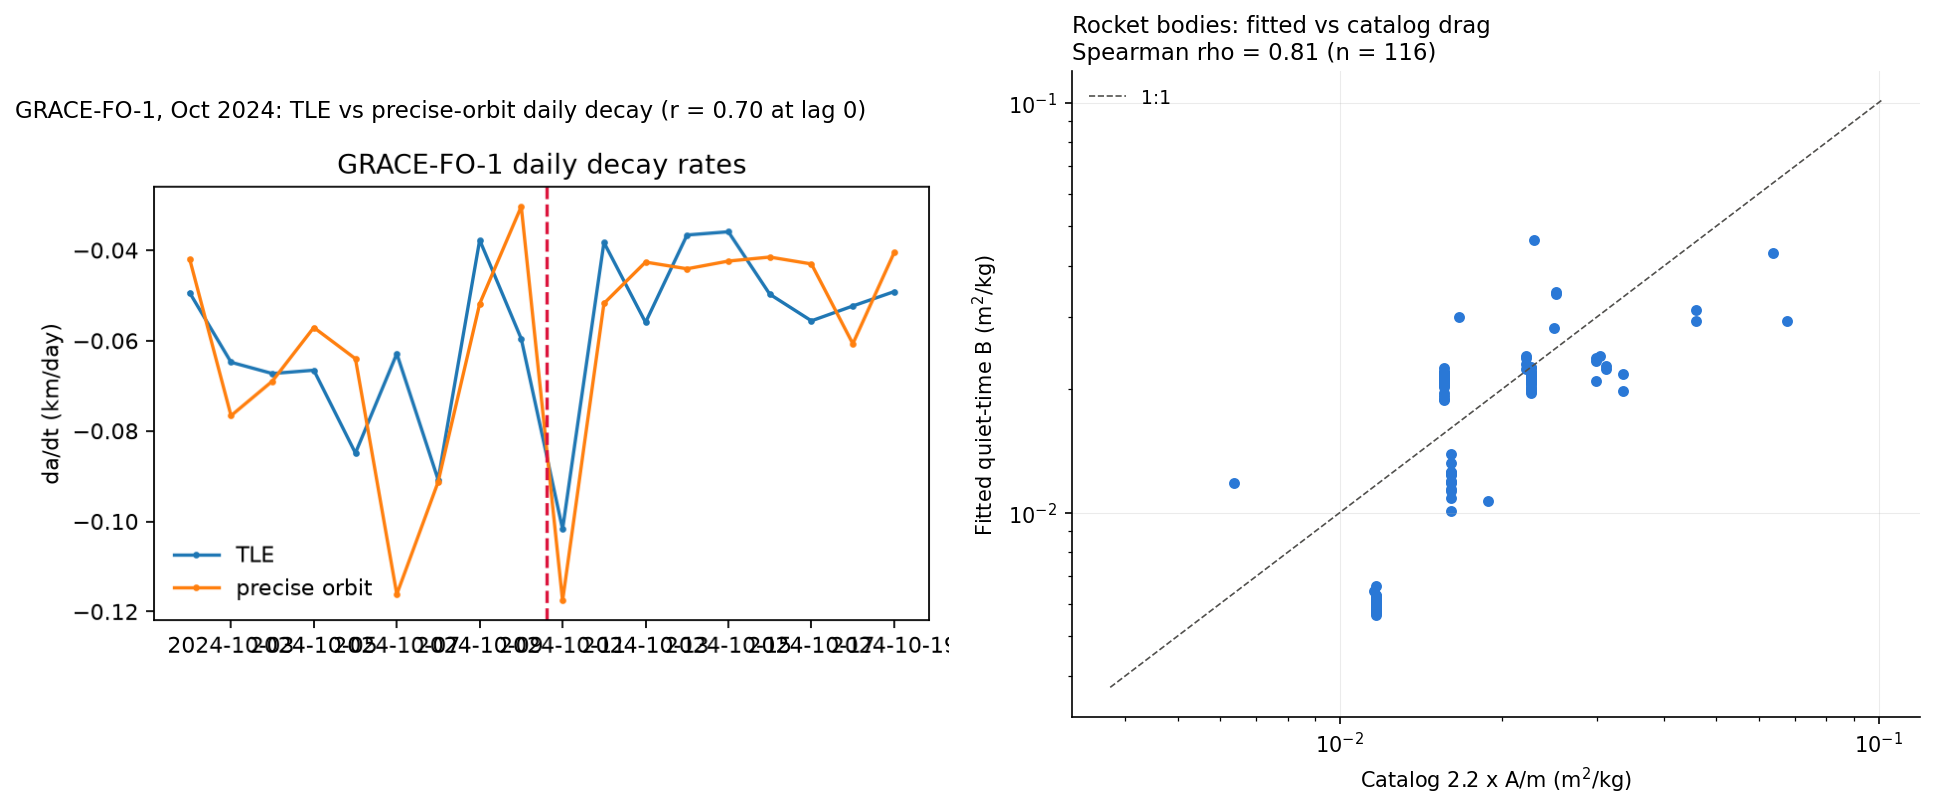
\includegraphics[width=\columnwidth]{fig6_validation.png}
\caption{Validation. Left: TLE-derived and precise-orbit decay rates of GRACE-FO-1 in October
2024 ($r=0.70$ at zero lag). Right: fitted drag sensitivity against the catalogue value for 116
rocket bodies (Spearman $\rho=0.81$).}
\label{fig:valid}
\end{figure}

\subsection{A simulator with a known answer}
We also built a simulator that integrates
Eq.~\eqref{eq:drag} through NRLMSIS~2.1 density for synthetic objects at 400--800~km. It plants
a storm boost of known size (by default $+50\%$ on days 0--2, gone by day 5), adds TLE-style
noise that triples during storms, and then runs everything through the same cleaning, fitting
and estimation code as the real data. With no noise the prediction follows the truth (median
error below 1\%), with no boost the residual is zero, and the planted boost is recovered inside
the event-study 95\% interval.
        % Sonu
\section{Causal Design and Estimators}
\label{sec:design}

\subsection{The causal graph}
Fig.~\ref{fig:dag} writes down what we assume. Solar activity raises both the UV flux (F10.7)
and the rate of storms (ap), and both of these raise density, which raises decay. Season and
altitude also affect decay. So we adjust for F10.7, its 81-day mean, season and altitude, and
we leave density alone because it is the path the storm acts through. Storms are set off by
solar-wind structures whose arrival nobody controls, which is what lets us treat each one as a
natural experiment. The causal reading rests on one assumption: once we adjust for this set,
nothing else that changes over time drives both storm timing and decay (for example an earlier
storm, or a change in tracking quality). The placebo dates, pre-trend test and high-altitude
control in Section~\ref{sec:robust} support this assumption but cannot prove it. Because passive
objects cannot manoeuvre, their response is purely physical.

\begin{figure}[t]
\centering
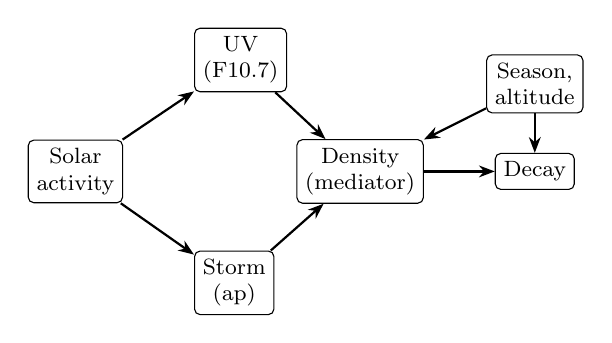
\begin{tikzpicture}[node distance=6mm and 9mm, every node/.style={font=\footnotesize},
  box/.style={draw, rounded corners=2pt, inner sep=3pt, align=center},
  arr/.style={-{Stealth[length=2mm]}, thick}]
\node[box] (sun) {Solar\\activity};
\node[box, above right=of sun] (uv) {UV\\(F10.7)};
\node[box, below right=of sun] (ap) {Storm\\(ap)};
\node[box, right=22mm of sun] (rho) {Density\\(mediator)};
\node[box, right=of rho] (y) {Decay};
\node[box, above=5mm of y] (sa) {Season,\\altitude};
\draw[arr] (sun) -- (uv); \draw[arr] (sun) -- (ap);
\draw[arr] (uv) -- (rho); \draw[arr] (ap) -- (rho);
\draw[arr] (rho) -- (y); \draw[arr] (sa) -- (y); \draw[arr] (sa) -- (rho);
\end{tikzpicture}
\caption{Causal graph. F10.7 confounds the storm--decay relation. Density is the mediator
through which storms act and is never controlled for.}
\label{fig:dag}
\end{figure}

\subsection{Stacked event study (Q1)}
For each storm $s$ we collect every interval whose
midpoint lies between days $-10$ and $+20$ of its onset. Storms are often less than 30 days
apart, so we drop a row from stack $s$ if it falls inside another storm's active window (three
days before that storm's onset to three days after its recovery end), and we drop a whole storm
if its day~0 is contaminated or too few clean days are
left~\cite{cengiz2019stacked,callaway2021did}. That leaves 12 of the 20 storms. On the stacked
rows we fit, by weighted least squares with weights $\Delta t$,
\begin{equation}
Y_{ist} = \alpha_{is} + \sum_{k\neq -1} \beta_k\,\mathbf{1}[\lfloor e_{st}\rfloor = k]
+ \gamma^\top X_t + \varepsilon_{ist},
\end{equation}
where $\alpha_{is}$ is an object-by-stack fixed effect, $e_{st}$ is the event day, day $-1$ is
the reference and $X_t$ holds the time-varying confounders (F10.7, its 81-day mean, season). Our
headline number is the mean of $\beta_0$, $\beta_1$ and $\beta_2$, i.e. days 0--2.

\subsection{Double machine learning (Q1)}
The event study tells us how much happens on storm days. Double machine learning
(DML)~\cite{chernozhukov2018dml} tells us how much happens per unit of storm strength, using the
partially linear model $Y = \theta T + g(X) + \varepsilon$. The treatment $T$ is the
interval-mean ap in nT. We use the mean rather than the total because storm intervals are
shorter, and the total would mix interval length into the effect. We estimate $E[Y\mid X]$ and
$E[T\mid X]$ with cross-fitting, regress the outcome residual on the treatment residual (weights
$\Delta t$), and report $\theta$ in m/day per nT. The folds are whole blocks of time (one storm
window, or one calendar week outside storms), never random rows. Random folds would let the
models memorise storm dates.

We fixed the model-selection rule before touching the real data. Each nuisance model is picked
from a straight line, a cautious XGBoost and a flexible XGBoost by its error on held-out storms,
so the data choose the model but not the rule. On synthetic data the full pipeline, selection
included, covers the true effect in 48 of 50 worlds with linear confounding and 49 of 50 with
curved confounding. A naive regression covers it in only 9 of 50 (bias $+149\%$). The main ap
lag is 0~h, and we also report 6, 12 and 24~h.

\subsection{Causal forest (Q2)}
A causal forest~\cite{wager2018forest,athey2019grf} (EconML CausalForestDML) uses the same
residuals and storm-blocked folds as DML but lets $\theta$ change with altitude, inclination and
drag sensitivity. We draw the effect on an altitude $\times$ drag-sensitivity grid and grey out
cells with fewer than three nearby objects. Since Eq.~\eqref{eq:drag} makes decay proportional
to $B$, we also fit the forest to $Y_{\text{total}}/\hat B$. On synthetic data the forest recovers the planted pattern
(correlation 0.925), and the map is stable across five seeds.

\subsection{Model-based offset ratio (Q3)}
No passive object flies near the Starlink shells (none at 440--570~km and 38--58$^\circ$), so
each satellite acts as its own control. For satellite $j$, storm $s$ and
window $w$, where the \emph{ducking} window runs from onset to recovery end and the
\emph{recovery} window covers the next ten days, the predicted and observed storm losses are
\begin{align}
P_{jsw} &= \textstyle\sum_{i\in w} (\hat B_j D_i - \hat B_j D_i^{\text{quiet}})\,\Delta t_i,\\
O_{jsw} &= \textstyle\sum_{i\in w} (\dot a_i^{\text{obs}} - \bar{\dot a}_{js}^{\text{pre}})\,\Delta t_i,
\end{align}
where $\bar{\dot a}^{\text{pre}}_{js}$ is the satellite's own mean decay over days $-10$ to
$-3$, so routine station keeping cancels out. The offset ratio is $1 - \sum O / \sum P$ over all
satellite--storm pairs. A value of 0 means the satellite lost everything physics predicts, and 1
means it lost nothing extra. The total splits neatly into a ducking part and a recovery part.

For $\hat B_j$ we take the catalogue value $2.2\,A/m$ and scale it by the median fitted/catalogue
ratio of rocket bodies within $\pm50$~km of each shell (0.71--0.77, against about 0.8 over all
rocket bodies). The corrected ratio also subtracts the passive objects' model error by storm
class and 100-km band. We exclude rows in deorbit (free drag) and rows in a 21-day window with
more than 1~km of net altitude change (orbit raising, shell changes), and each storm's windows
stop at the next storm's onset so no storm is counted twice.

\subsection{Extreme-storm check (Q1)}
TLEs smear out fast changes, so for the three largest storms we therefore also measure the total altitude lost
from the last calm day before the storm (in days $-10$ to $-3$) to the first calm day after
recovery, where calm means every 3-hour ap is below 27. We compare observed with predicted loss
and subtract the model's own local quiet error. We fixed the rule in advance: a storm counts as
a real model overshoot only if its days 0--3 over-prediction survives 3-day smoothing
\emph{and} the calm-to-calm loss is over-predicted against both baselines.

\subsection{Inference}
Every object sees the same storm, so our real sample size is 20 storms, not 178,107 rows. The
event-study, DML and offset-ratio intervals therefore cluster by storm (or quiet time block) and
use a wild cluster bootstrap with Webb weights~\cite{cameron2008bootstrap,webb2023wild}. Because
storms can sit close together, one row can end up in two event-study stacks, so the event
study's main test is a placebo test on 500 randomly drawn storm-free dates. Two intervals do not
cluster by storm. The causal forest's intervals treat rows as independent, so we read the forest
for its pattern only, and the calm-to-calm intervals resample objects within one storm. All
intervals are conditional on the fitted drag sensitivities, and the offset-ratio intervals also
hold the predicted storm loss fixed. Every headline is also reported without the May and October
2024 storms (three storm entries: early May, the May superstorm and October).
  % Anil
\section{Q1: Storm Effect and Model Error}
\label{sec:q1}

\subsection{How much faster do objects fall?}
\label{sec:eventstudy}
Fig.~\ref{fig:es} shows the event study on the main sample (178,107 intervals, 12 clean
storms). Before onset the coefficients wander around zero (placebo pre-trend test $p=0.41$). On day~0 the total
storm effect is about $-30$~m/day and on day~1 about $-12$~m/day. By day~2 it is close to zero,
although days 4 and 5 dip slightly again (about $-5$ and $-7$~m/day). Averaged over days 0--2,
the total storm effect is $-14.1$~m/day (95\% CI $-19.8$ to $-8.4$). Against a pooled quiet-time
mean of about $-50$~m/day, that is roughly 28\% faster decay (Table~\ref{tab:q1}). None of 500
placebo storm dates gives an effect this large ($p<0.002$).

DML tells the same story per unit of storm strength: $\theta = -0.393$~m/day per nT of ap (95\%
CI $-0.527$ to $-0.268$), or $-39$~m/day per 100~nT. A typical day~0 has a mean ap of 57~nT
against a quiet 7~nT, which works out to about $-20$~m/day, in line with the event study. For
$Y_{\text{total}}$, naive regression, linear controls and DML agree to within 1\%. The outcome
already subtracts NRLMSIS run with the real F10.7, so little UV confounding is left. On synthetic data, where UV error goes straight
into the outcome, the naive estimate is biased by more than $+100\%$ and DML is not.

\begin{figure}[t]
\centering
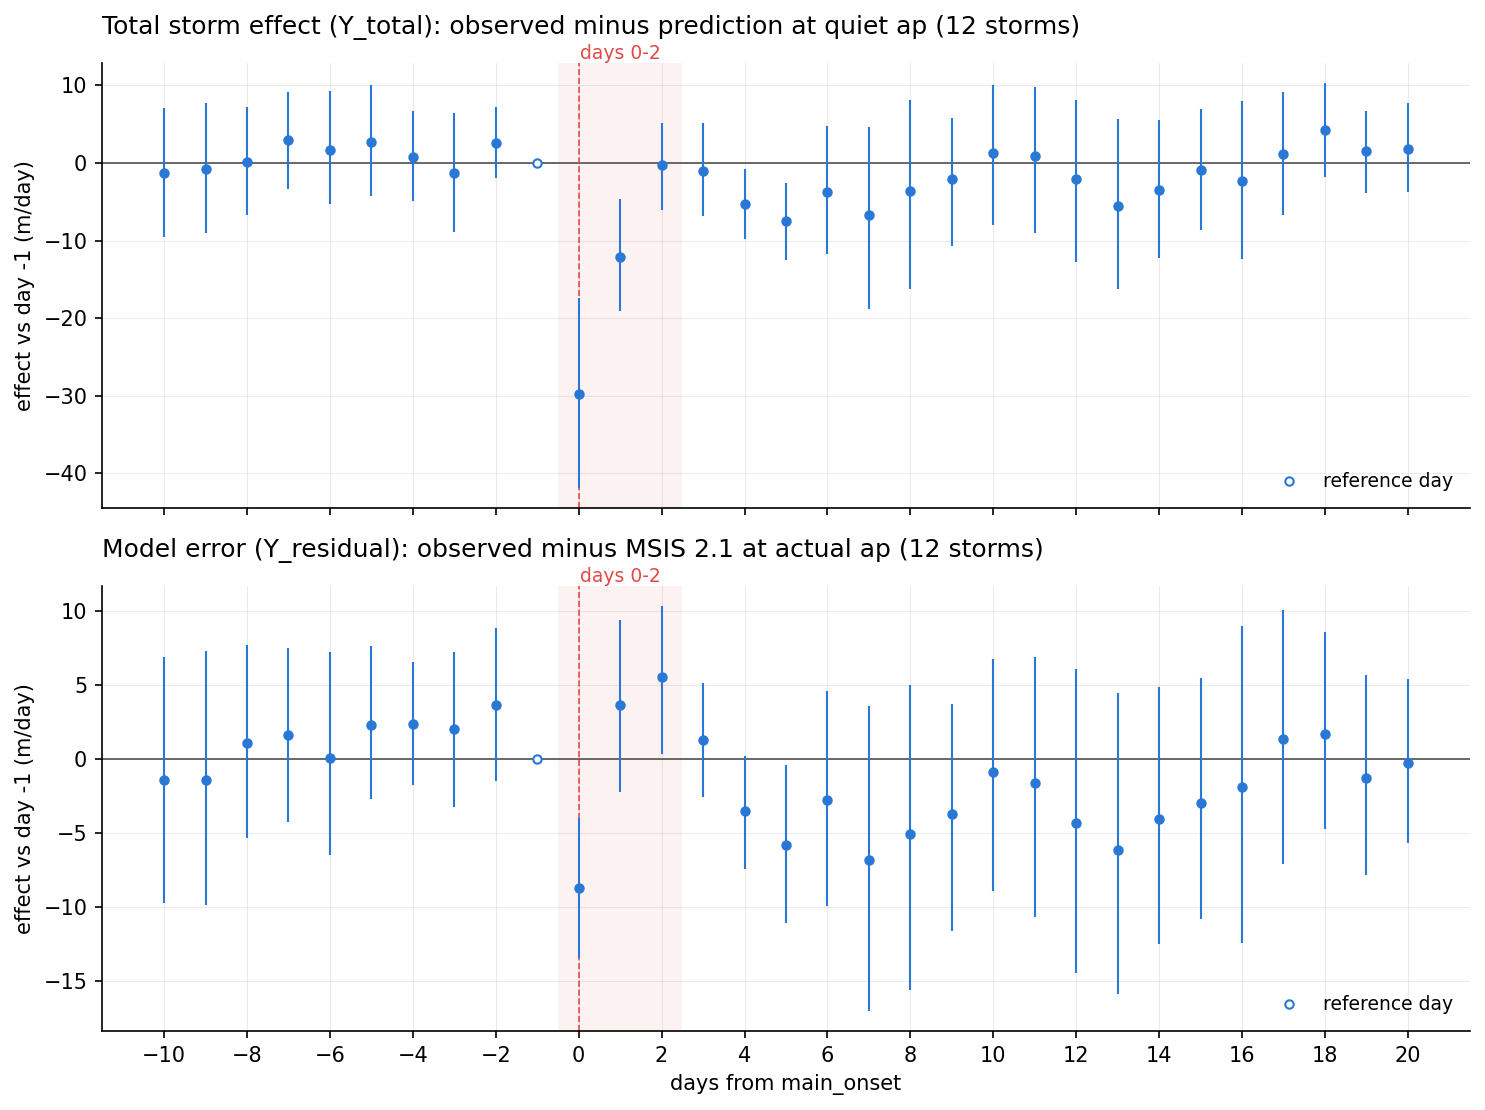
\includegraphics[width=\columnwidth]{fig4_event_study.png}
\caption{Stacked event study (12 clean storms, 95\% storm-clustered intervals). Top: total
storm effect $Y_{\text{total}}$. Bottom: model error $Y_{\text{residual}}$. Day $-1$ is the
reference, and the shaded band marks days 0--2.}
\label{fig:es}
\end{figure}

\begin{table}[t]
\caption{Q1 estimates (m/day; DML in m/day per nT of ap)}
\label{tab:q1}
\centering
\small
\begin{tabular}{@{}lcc@{}}
\toprule
 & $Y_{\text{total}}$ & $Y_{\text{residual}}$ \\
\midrule
Event study, days 0--2 & $-14.1$ & $+0.2$ \\
 & {\scriptsize($-19.8$, $-8.4$)} & {\scriptsize($-3.2$, $+3.2$)} \\
\quad placebo $p$ & $<0.002$ & 0.88 \\
\quad without May/Oct 2024 & $-13.9$ & $-2.2$ \\
 & {\scriptsize($-16.6$, $-10.9$)} & {\scriptsize($-4.4$, $0.0$)} \\
\quad stricter clean rule & $-10.1$ & $+1.4$ \\
 & {\scriptsize($-14.0$, $-6.2$)} & {\scriptsize($-2.5$, $+5.4$)} \\
DML, per nT & $-0.393$ & $-0.050$ \\
 & {\scriptsize($-0.527$, $-0.268$)} & {\scriptsize($-0.141$, $+0.047$)} \\
\quad without May/Oct 2024 & $-0.503$ & $-0.152$ \\
 & {\scriptsize($-0.642$, $-0.361$)} & {\scriptsize($-0.267$, $-0.042$)} \\
\bottomrule
\end{tabular}
\end{table}

The result does not lean on the two biggest storms. Without May and October 2024 the event study
gives $-13.9$~m/day, and DML per nT is actually larger ($-0.503$). Per nT, the total effect is
similar in moderate, strong and severe storms (about $-0.6$~m/day per nT) and smaller in the
single extreme storm (about $-0.25$). That hints at saturation, but with only three large storms
the difference is not significant at the storm level (permutation $p=0.45$).

\subsection{Is NRLMSIS 2.1 wrong during storms?}
\label{sec:modelerror}
On average, not by much, but the average hides a timing problem. Pooled over days 0--2 the
event-study model error is $+0.2$~m/day (95\% CI $-3.2$ to $+3.2$), and the change in the
residual from days $-10..-3$ to days $0..3$, averaged over all 20 storms, is $+0.8$~m/day (CI
$-5.8$ to $+7.4$). Look at Fig.~\ref{fig:es} (bottom), though, and there is a negative error of
about $-9$~m/day on day~0, balanced by small positive errors on days 1--2. DML by storm class
pins this down. In moderate storms the model error is $-0.133$~m/day per nT (95\% CI $-0.247$
to $-0.010$), and in strong storms $-0.210$ (CI $-0.348$ to $-0.068$). In other words, at peak
ap objects lose more altitude than NRLMSIS~2.1 predicts.

There is also a hint of the opposite error a little later. A positive model error 12--24~h after
high ap (24~h lag: $+0.117$, CI $0.035$ to $0.200$) would mean the model keeps the storm
atmosphere around for too long. But it disappears once May and October 2024 are removed (24~h:
$+0.048$, CI $-0.055$ to $+0.152$), so we do not claim it as a general result.

\subsection{The three largest storms}
\label{sec:extreme}
The severe and extreme storms each went wrong in their own way (Fig.~\ref{fig:extreme}).

\textit{October 2024} (severe) is a real model overshoot. The days 0--3 over-prediction survives
3-day smoothing ($+28.4$~m/day, CI $+22.8$ to $+33.9$). From calm day to calm day, objects lost
only 0.86 (CI 0.84--0.87) of the predicted altitude, or $+169$~m once the model's local quiet
error is removed, and this holds in every 100-km band (0.85--0.90).

\textit{May 2024} (extreme) looks like a timing error rather than a wrong total. The early excess
survives smoothing ($+6.9$~m/day), but the calm-to-calm loss is not over-predicted. Against the
model's local quiet error ($\pm30$ days) the difference is $-1$~m (CI $-10$ to $+7$), and against
its pre-storm error the model actually under-predicts the loss by 75~m (CI 59 to 92). So the
model put about the right total, or slightly too little, on the wrong days. The raw ratio of 0.91
comes from an over-prediction that was already there before the storm began.

\textit{December 2024} (severe) goes the other way. Objects lost 1.19 (CI 1.17--1.22) times the
predicted altitude, so here the model under-predicts.

Moving the calm day after the storm two or three days later changes these ratios by at most
0.02, and the high-altitude control differs from its prediction by at most 7~m. So in October and
December the NRLMSIS~2.1 error is 14--19\% of the total calm-to-calm loss (storm plus background
decay), in May it is close to zero once the quiet error is removed, and its sign changes from
storm to storm. No single correction factor would fix all three.

\begin{figure*}[t]
\centering
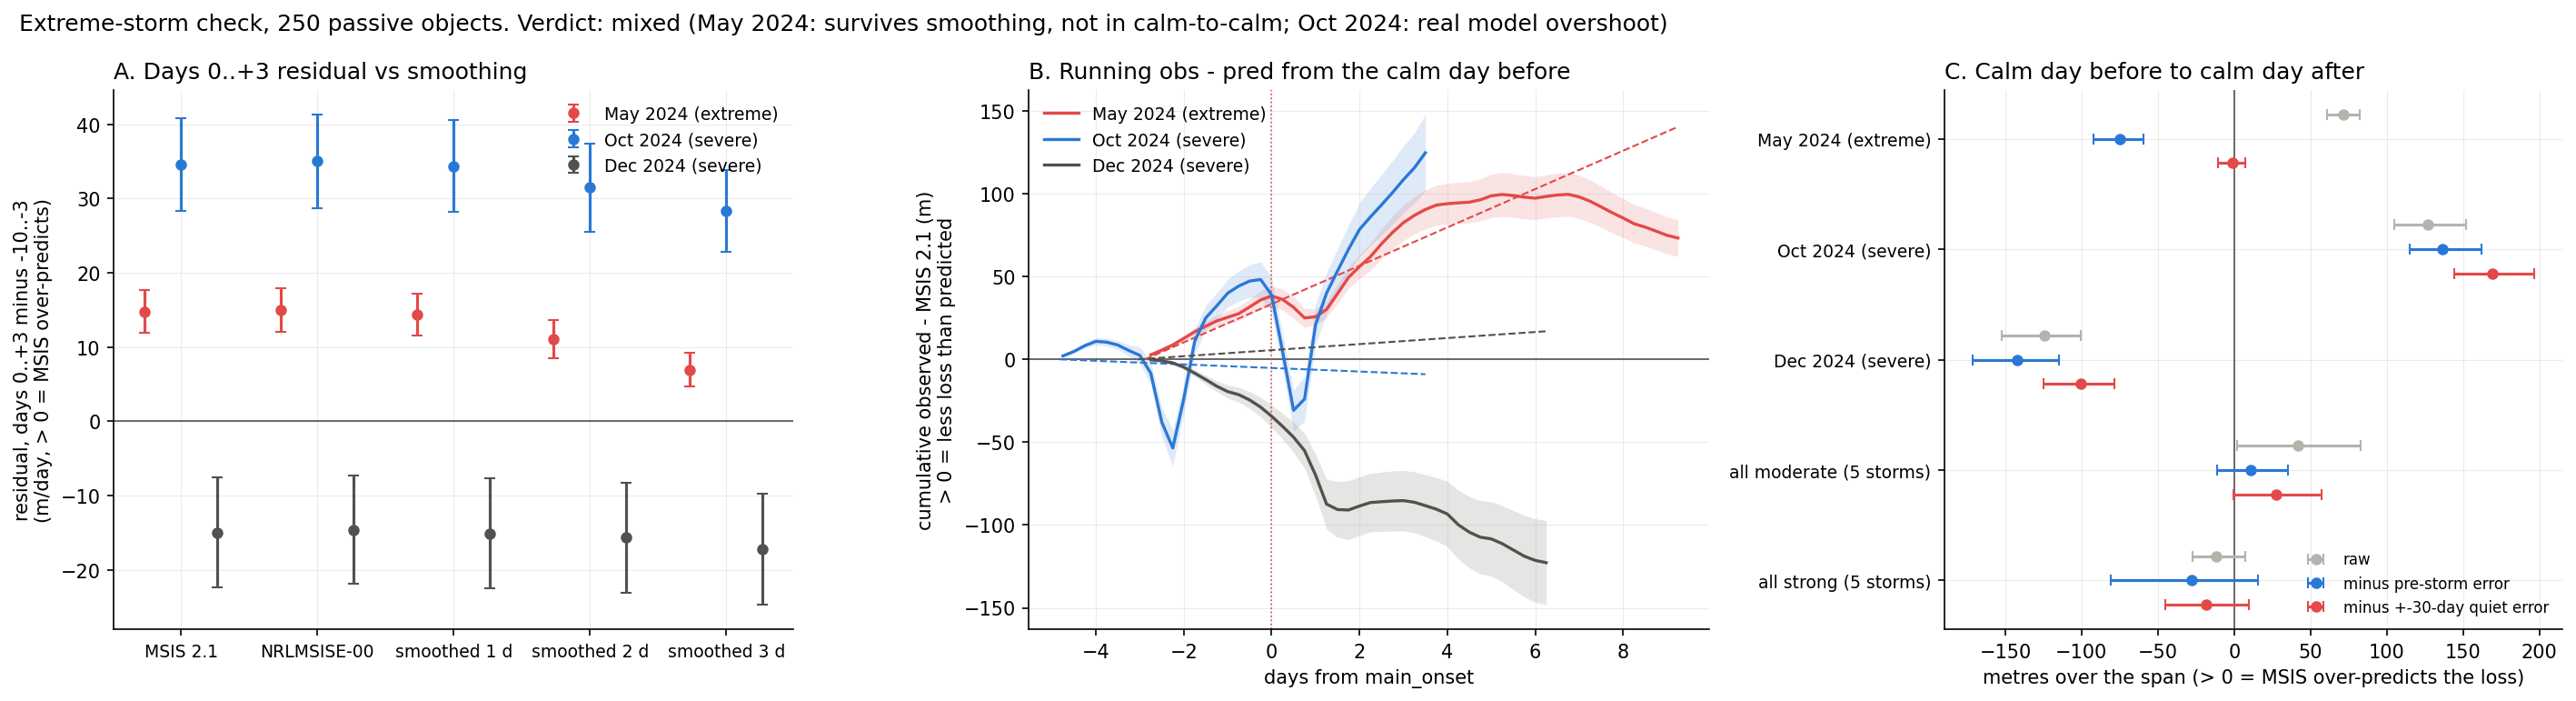
\includegraphics[width=\textwidth]{fig8_extreme_check.png}
\caption{The three largest storms (250 passive objects). (A) Days 0--3 residual change, raw and
smoothed over three days. (B) Running observed minus predicted altitude loss from the calm day
before; dashed: the pre-storm error carried forward. (C) Calm-to-calm loss, observed over
predicted: May 0.91, October 0.86, December 1.19.}
\label{fig:extreme}
\end{figure*}
% Anil (event study) + Holla (DML) + Sonu (extreme storms)
\section{Q2: Who Is Hit Hardest?}
\label{sec:q2}

Fig.~\ref{fig:vuln} shows the causal forest for $Y_{\text{total}}$ on the 250 passive objects.
Drag sensitivity dominates the variable importance (0.892), well ahead of altitude (0.101) and
inclination (0.007), and the map barely changes across five forest seeds (minimum correlation
0.986). Seed stability tells us the algorithm is repeatable, not that the map would hold for new
storms. The first finding is no surprise given Eq.~\eqref{eq:drag}: in m/day, a large, light
object always loses more than a small, dense one.

The more interesting map is the effect per unit drag sensitivity (Fig.~\ref{fig:vuln}C). With
size divided out, altitude takes almost all the importance (0.993, against 0.005 for inclination
and 0.002 for drag sensitivity, with seed stability 0.995), and within each altitude row the map
is flat. So the storm effect is simply proportional to drag sensitivity, multiplied by an
altitude factor. That factor falls from $-10.8$ at 617~km to $-3.7$ at 747~km
((m/day per nT) per m$^2$/kg), about 2.9-fold over 130~km, or roughly one e-fold every
100--120~km. That is the same order as a thermospheric density scale height, which is a good sign
the map reflects real physics. As a cross-check, dividing the $Y_{\text{total}}$ map by drag
sensitivity cell by cell reproduces the per-drag forest (correlation 0.96). In this cohort,
inclination adds little once the response is averaged over an orbit.

The forest's intervals treat rows as independent, so we read the
map for its shape and take the size of the effect from DML. We do not interpret cells that rest
on a single group of objects (519 and 779~km).

\begin{figure*}[t]
\centering
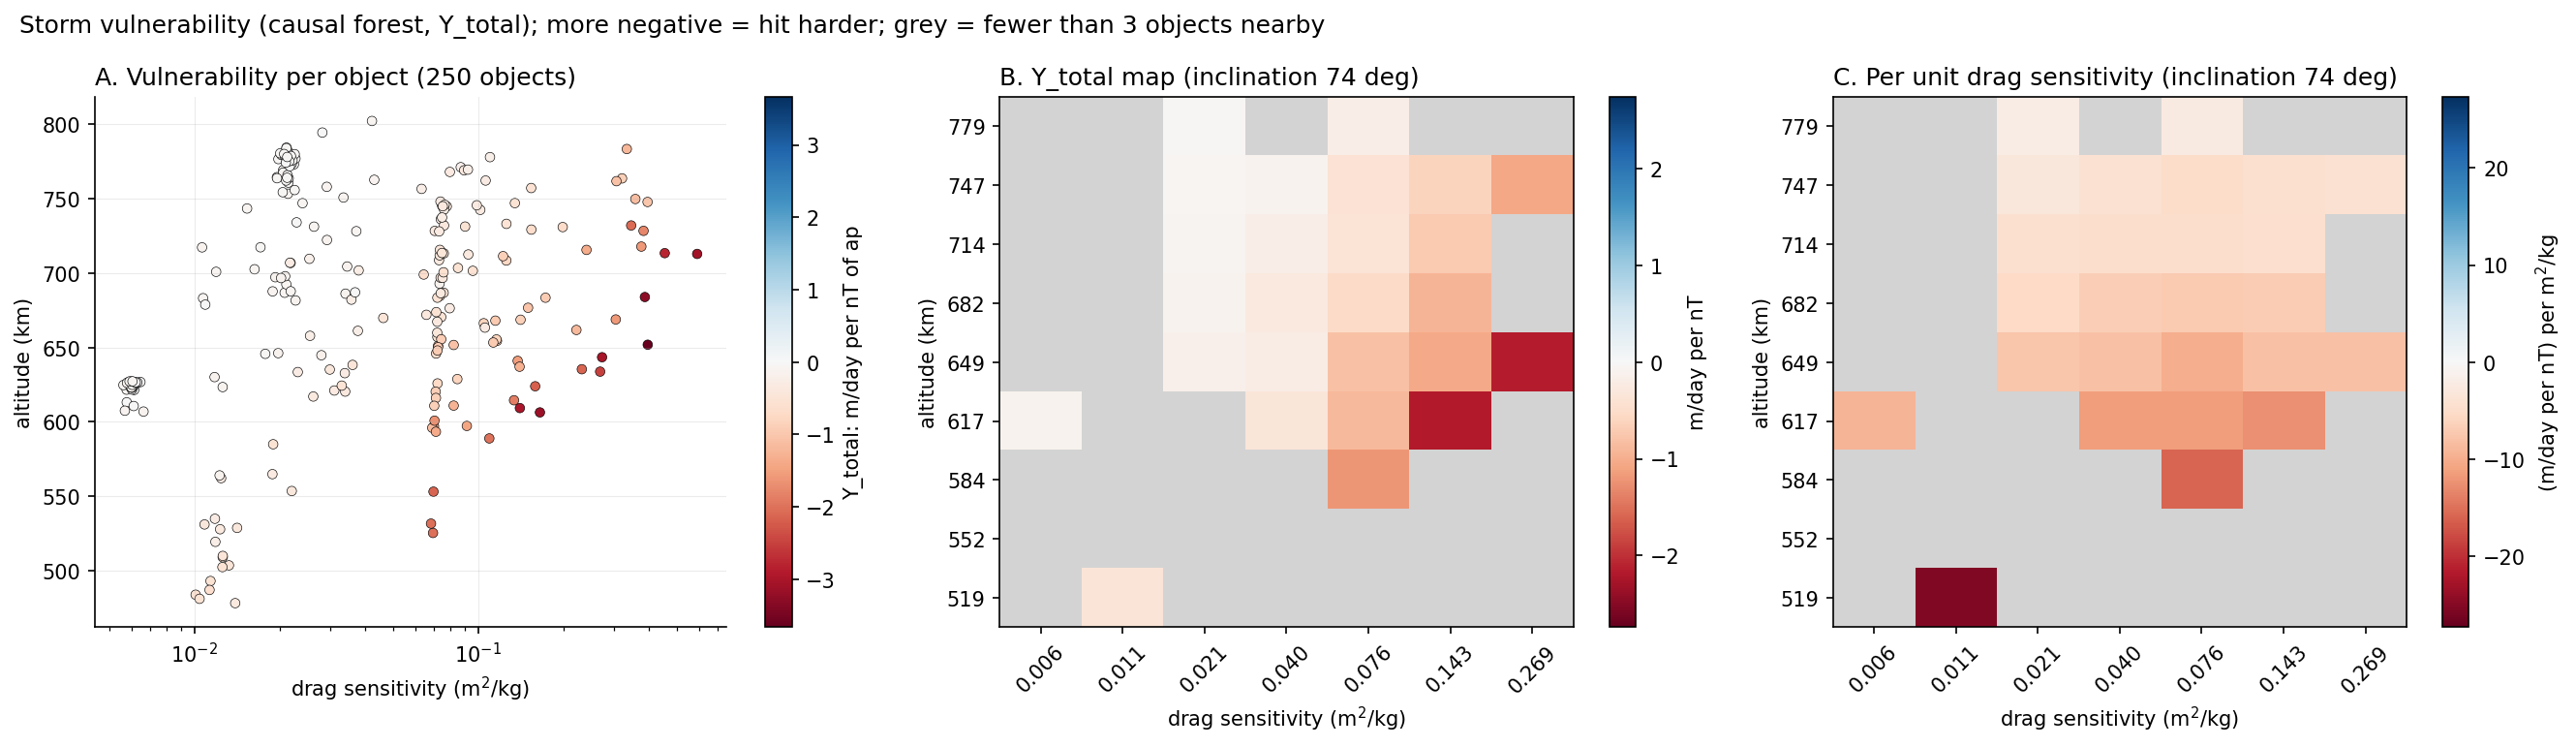
\includegraphics[width=\textwidth]{fig9_vulnerability.png}
\caption{Storm vulnerability (causal forest, 250 passive objects, m/day per nT of ap).
(A) Per-object effect. (B) Effect on an altitude $\times$ drag-sensitivity grid at the median
inclination. (C) Effect per unit drag sensitivity. Grey cells have fewer than three nearby
objects.}
\label{fig:vuln}
\end{figure*}
% Holla
\section{Q3: Do Operators Fight Back?}
\label{sec:q3}

In the active cohort, 26 satellites showed manoeuvres: the 25 Starlinks and one 1967
calibration satellite whose ``manoeuvres'' turned out to sit on steady free-drag decay, which the
free-drag screen removes. Question~3 is therefore an exploratory Starlink study. After the
screens, 21 Starlinks contribute across the 20 storms. Coverage is uneven, because not every
satellite covers every storm's windows.

Table~\ref{tab:q3} and Fig.~\ref{fig:offset} give the result. With the passive model-error
correction, the offset ratio is 1.17 (95\% CI 0.97--1.36). At the point estimate, Starlinks lose
no more altitude around storms than in their normal pre-storm routine, and the interval still
allows an offset slightly short of complete. Almost all of it happens during the storm (ducking
part 1.16, CI 1.05--1.27), while the recovery part is about zero ($+0.01$, CI $-0.22$ to
$+0.21$). At TLE resolution, then, the satellites make up the loss while the storm is still
going, not by climbing back afterwards.

The result holds without May and October 2024 (1.25, CI 1.08--1.41) and without the six storms
whose pre-storm quiet ap was raised by an earlier storm (1.15, CI 1.04--1.26). In that second
subset the recovery part is $+0.15$ (CI 0.04--0.28), so a small part of the offset may happen
after the storm. Values above 1 are larger than the scatter on storm-free dates and could mean
slightly over-compensating thrust or the smoothing in mean-element TLEs. Since the lower end of
the main interval is just below 1, our reading is careful: for the selected satellites and
operating periods, the observed orbit changes are consistent with an approximately complete
offset of the model-predicted storm loss. An offset ratio is not a measurement of thrust. TLEs
alone cannot separate thrust, attitude changes, routine manoeuvre timing and model error.

\begin{table}[t]
\caption{Starlink operator offset ratio (21 satellites)}
\label{tab:q3}
\centering
\small
\begin{tabular}{@{}lcc@{}}
\toprule
Run & Offset & 95\% CI \\
\midrule
All 20 storms, uncorrected & 1.19 & 0.77--1.64 \\
All 20 storms, corrected & \textbf{1.17} & 0.97--1.36 \\
\quad ducking part & 1.16 & 1.05--1.27 \\
\quad recovery part & $+0.01$ & $-0.22$ to 0.21 \\
Without May/Oct 2024 & 1.25 & 1.08--1.41 \\
Undisturbed quiet ap (14 storms) & 1.15 & 1.04--1.26 \\
\bottomrule
\end{tabular}
\end{table}

\begin{figure}[t]
\centering
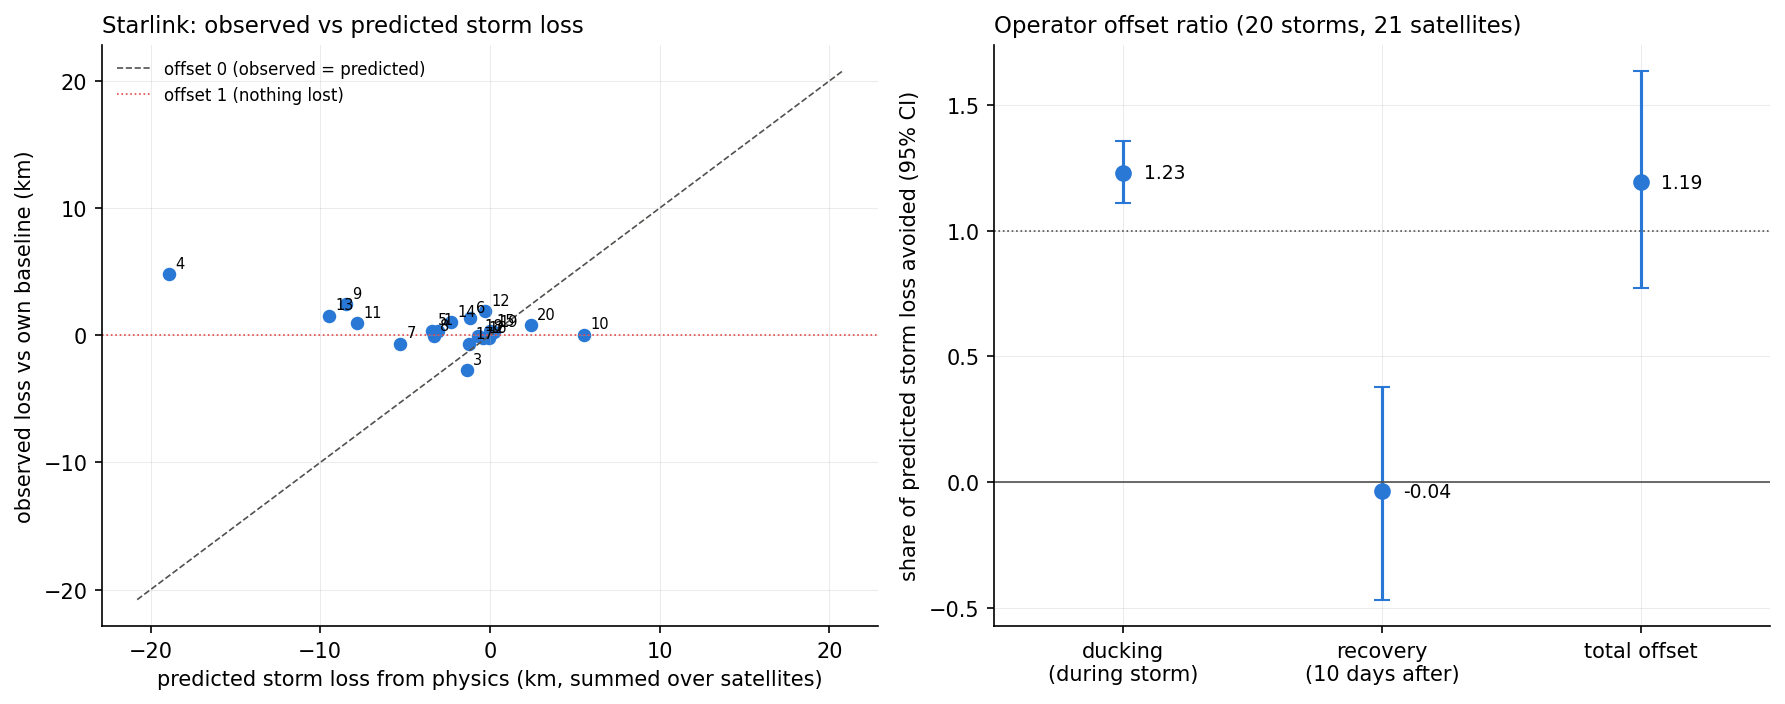
\includegraphics[width=\columnwidth]{fig7_operator_offset.png}
\caption{Starlink offset (uncorrected run: total 1.19, ducking 1.23, recovery $-0.04$; the
corrected values are in Table~\ref{tab:q3}). Left: observed against predicted storm loss per
storm, summed over satellites; points near the dotted line lost nothing. Right: ducking, recovery
and total offset with 95\% storm-clustered intervals.}
\label{fig:offset}
\end{figure}

Five caveats apply. First, this is one operator. Second, drag sensitivity comes from the
catalogue scaled by passive-object fits. In a pre-freeze run, scaling it by $\pm25\%$ moved the
ratio to 1.15--1.25, but a badly wrong scale could fake an offset. Third, the screens that drop
deorbits and orbit raises are based on observed altitude, so they could also drop periods of poor
compensation. Fourth, the passive model-error correction is carried over in m/day by storm class
and altitude band, not scaled to each satellite's drag sensitivity. Fifth, the intervals hold the
predicted loss fixed, and a placebo on Starlinks in free drag is compatible with zero but too
imprecise to really validate the method.
      % Anil
\section{Trying to Break the Results}
\label{sec:robust}

For each result we ran tests that could have knocked it down (Table~\ref{tab:checks}), though
they do not back every result equally.

The high-altitude control group (15 objects at 1,040--1,211~km, where storm heating barely
reaches) gives a small DML effect of $-0.023$~m/day per nT (CI $-0.026$ to $-0.021$). That is
not exactly zero, but it is about 6\% of the main estimate and inside an equivalence band of
$\pm0.197$ (half the main estimate) that we set in advance. Adding a random common cause moves
the DML estimate by $-0.01$ standard errors, which shows numerical stability rather than
robustness to a real missing confounder. Shifting the storm calendar to 100 random wrong dates
gives a mean effect of $+0.004$ (SD 0.028), and none of the 100 shifts matches the real estimate
($p=0.010$). Dropping the intervals flagged as TLE climbs moves the event-study effect only from
$-14.1$ to $-14.6$~m/day. The synthetic tests show that the pipeline works in simulated worlds,
not that the real causal assumptions hold.

\begin{table}[t]
\caption{Checks behind each result}
\label{tab:checks}
\centering
\small
\begin{tabular}{@{}p{3.1cm}p{3.0cm}c@{}}
\toprule
Check & Result & \\
\midrule
Placebo storm dates (500) & $p<0.002$ & pass \\
Pre-trend (days $-10..-2$) & $p=0.41$ & pass \\
High-altitude control, ES & $-0.69$ ($-1.42$, $0.07$) & pass \\
High-altitude control, DML & $-0.023$, inside $\pm0.197$ & pass \\
Random common cause & $-0.01$ SE & pass \\
Shuffled storm timing (100) & $p=0.010$ & pass \\
Without May/Oct 2024 & $-13.9$ (ES), $-0.503$ (DML) & pass \\
No Hampel filter (ES) & $-16.0$ ($-23.4$, $-8.3$) & pass \\
Q3 screen 0.5 / 2~km & 1.18 / 1.18 & pass \\
Synthetic DML coverage & 48/50, 49/50 & pass \\
Synthetic forest recovery & $r=0.925$ & pass \\
Held-out quiet residual & $-0.13$ (SE 1.07) & pass \\
GRACE-FO decay rate & $r=0.70$ & good \\
Swarm-A decay rate & $r=0.457$ & fair \\
Catalogue drag ranking & $\rho=0.81$ & good \\
\bottomrule
\end{tabular}
\end{table}

For the model error $Y_{\text{residual}}$ the evidence is weaker. The shuffled-timing placebo
gives $p=0.059$ and the pooled DML interval covers zero, which is why we do not claim a pooled
per-nT model error and report the class-specific estimates instead
(Section~\ref{sec:modelerror}).

\textit{Does the outlier filter shape the answer?} The Hampel filter works on the NRLMSIS~2.1
residual, so it might throw away real storm-time errors along with bad TLEs. Removal is concentrated at onset: it flags 18.8\% of day-0 rows against
4.0\% on days $-10..-3$ and 5.5\% overall, and the day-0 share is highest in severe storms
(43.7\%). Rerunning the event study with the flagged rows put back gives $-16.0$~m/day (CI $-23.4$ to
$-8.4$), with no filter at all $-16.0$ (CI $-23.4$ to $-8.3$), and with $k=5$ $-15.2$ (CI $-21.4$
to $-8.7$). In every version the model error stays near zero ($-0.3$~m/day, CI $-5.2$ to $+4.3$ with
the rows put back). So the filter makes our headline slightly smaller, not larger,
and no headline moves by more than 20\%.

Likewise, tightening the Q3 orbit-change screen from 1~km to 0.5~km or loosening it to 2~km
gives an offset of 1.18 both times (against 1.17), and only the number of satellite--storm pairs
changes (262, 278 and 286).
     % Holla
\section{Discussion and Limitations}
\label{sec:discussion}

Put together, the results describe a short, sharp shock. On the onset day a typical storm makes
objects fall roughly 60\% faster ($-30$ against a pooled quiet mean of about $-50$~m/day). Most of
the response comes near onset, with smaller negative values still visible on days 4--5. Pooled
over days 0--2, NRLMSIS~2.1 shows little mean error, but that average hides two problems. In
ordinary storms it gets the timing wrong and under-predicts decay at peak ap, and in the largest
storms its totals are wrong in storm-specific ways. That matters more for short-term conjunction
screening than for lifetime estimates. Vulnerability follows the drag equation: drag sensitivity
times an altitude factor, with lower objects hit harder per unit drag. And in our exploratory
look at Starlink, the observed orbit changes are consistent with an approximately complete
offset of the predicted loss, almost all during the storm.

The study has clear limits, and we list eight. (1) One year of data gives 20 storms, of which 12
have clean event-study windows, so storm-level intervals are wide and class comparisons have
little power. (2) TLEs are mean-element fits, not true altitudes, and they blur changes faster
than about a day. This is why the extreme storms needed the calm-to-calm check. (3) Question~3
covers a single operator, with catalogue-scaled drag sensitivity and a weak placebo. (4) For six
storms the pre-storm quiet ap was raised by an earlier storm. A storm-free quiet ap would fix
this, and in its place we report the run without those storms. (5) The causal forest's intervals
treat rows as independent. (6) We only evaluate NRLMSIS, and other models such as JB2008 or DTM
may behave differently. (7) The Hampel filter runs on the NRLMSIS~2.1 residual and removes
proportionally more rows at storm onset. Our sensitivity runs show the headlines survive without
it, but the filter could still hide some real storm-peak model error. (8) Intervals are
conditional on the fitted drag sensitivities and, for Question~3, on the catalogue scaling, and
this uncertainty is not carried through. Natural next steps are held-out storms, more of the solar cycle, a
second constellation and other density models.
     % Holla
\section{Conclusion}
\label{sec:conclusion}

We set out to measure how much geomagnetic storms speed up the decay of objects in low Earth
orbit, using one year of public orbit data and treating each storm as a natural experiment. The
estimate is causal under the assumption that no time-varying confounding remains after we adjust
for F10.7 and season. Storms speed up decay by 14.1~m/day over days 0--2 after onset
(0.39~m/day per nT of ap), about 28\% faster than quiet-time decay, and the estimate holds
without the two largest storms and without the outlier filter. Over days 0--2, NRLMSIS~2.1 shows
little pooled error in ordinary storms but under-predicts decay at peak activity, and in the
largest storms its errors change sign from one storm to the next. Vulnerability scales with drag
sensitivity times an altitude factor that falls about threefold from 620 to 750~km. In an
exploratory analysis, Starlink orbit changes are consistent with an approximately complete
offset of the predicted storm loss (1.17, 95\% CI 0.97--1.36), almost all during the storm. The
storm effect is backed by placebo dates, a pre-trend test, a high-altitude control group and a
simulator with a known answer. The vulnerability map is backed by seed stability and synthetic
recovery. The offset ratio is backed only by subset checks, because its placebo is imprecise.

\section*{Author Contributions}
P.~Shiv built the orbit cohort, TLE cleaning and precise-orbit validation. S.~Akash built the
space-weather data and storm catalogue, the physics baseline and outcomes, the physics simulator,
the object catalogue, the active-satellite table, the model-based offset ratio and the
extreme-storm check. S.~Anil designed the analysis-table schema and causal graph and built the
synthetic data, the stacked event study and its checks, and the overlap correction of the offset
model. S.~Holla built the double machine learning, refutations, storm-class analysis and
vulnerability maps. All authors wrote the paper.

\section*{Code and Data Availability}
All inputs are public: TLEs from Space-Track, space weather from NASA OMNIWeb, object data from
CelesTrak and ESA DISCOSweb, and precise orbits from the GRACE-FO and Swarm missions. The code
(Python) and the processed analysis table are provided in the project submission folder. The
notebook \texttt{ICARUS\_final.ipynb} reproduces every headline number and figure from the
processed table; the raw-data download and table build are listed step by step in the
repository README.
     % Sonu

\bibliographystyle{IEEEtran}
\bibliography{refs}

\end{document}
